\chapter{Retrieval-Augmented Generation}

Retrieval-Augmented Generation (RAG) is the process of optimizing the output of a large language model, 
so it references an authoritative knowledge base outside of its training data sources before generating 
a response. Large Language Models (LLMs) are trained on vast volumes of data and use billions of parameters 
to generate original output for tasks like answering questions, translating languages, and completing 
sentences. RAG extends the already powerful capabilities of LLMs to specific domains or an organization's 
internal knowledge base, all without the need to retrain the model. It is a cost-effective approach 
to improving LLM output so it remains relevant, accurate, and useful in various contexts.

%+++++++++++++++++++++++++++++++++++++++++++
\section{Overview}
%-------------------------------------------




%+++++++++++++++++++++++++++++++++++++++++++
\subsection{Why is RAG important?}

LLMs are a key artificial intelligence (AI) technology powering intelligent chatbots and other natural 
language processing (NLP) applications. The goal is to create bots that can answer user questions in 
various contexts by cross-referencing authoritative knowledge sources. Unfortunately, the nature of 
LLM technology introduces unpredictability in LLM responses. Additionally, LLM training data is static 
and introduces a cut-off date on the knowledge it has.

Known challenges of LLMs include:

\begin{itemize}
%\setlength{\itemsep}{0pt}
%\setlength{\parsep}{0pt}
\setlength{\parskip}{0pt}
\item[-]
Presenting false information when it does not have the answer.

\item[-]
Presenting out-of-date or generic information when the user expects a specific, current response.

\item[-]
Creating a response from non-authoritative sources.

\item[-]
Creating inaccurate responses due to terminology confusion, wherein different training sources use 
the same terminology to talk about different things.
\end{itemize}

You can think of the Large Language Model as an over-enthusiastic new employee who refuses to stay 
informed with current events but will always answer every question with absolute confidence. Unfortunately, 
such an attitude can negatively impact user trust and is not something you want your chatbots to emulate!

RAG is one approach to solving some of these challenges. It redirects the LLM to retrieve relevant 
information from authoritative, pre-determined knowledge sources. Organizations have greater control 
over the generated text output, and users gain insights into how the LLM generates the response.


%+++++++++++++++++++++++++++++++++++++++++++
\subsection{Benefits of RAG}

RAG technology brings several benefits to an organization's generative AI efforts.

\subsubsection{Cost-effective implementation}

Chatbot development typically begins using a foundation model. Foundation models (FMs) are API-accessible 
LLMs trained on a broad spectrum of generalized and unlabeled data. The computational and financial 
costs of retraining FMs for organization or domain-specific information are high. RAG is a more cost-effective 
approach to introducing new data to the LLM. It makes generative artificial intelligence (generative 
AI) technology more broadly accessible and usable.

\subsubsection{Current information}

Even if the original training data sources for an LLM are suitable for your needs, it is challenging 
to maintain relevancy. RAG allows developers to provide the latest research, statistics, or news to 
the generative models. They can use RAG to connect the LLM directly to live social media feeds, news 
sites, or other frequently-updated information sources. The LLM can then provide the latest information 
to the users.

\subsubsection{Enhanced user trust}

RAG allows the LLM to present accurate information with source attribution. The output can include 
citations or references to sources. Users can also look up source documents themselves if they require 
further clarification or more detail. This can increase trust and confidence in your generative AI 
solution.

\subsubsection{More developer control}

With RAG, developers can test and improve their chat applications more efficiently. They can control 
and change the LLM's information sources to adapt to changing requirements or cross-functional usage. 
Developers can also restrict sensitive information retrieval to different authorization levels and 
ensure the LLM generates appropriate responses. In addition, they can also troubleshoot and make fixes 
if the LLM references incorrect information sources for specific questions. Organizations can implement 
generative AI technology more confidently for a broader range of applications.


%+++++++++++++++++++++++++++++++++++++++++++
\subsection{Principles of RAG}

RAG is a generative AI technology that combines the capabilities of LLMs with the knowledge retrieval 
capabilities of search engines. It uses a two-step process to generate responses to user queries: 
retrieval and generation.

\subsubsection{Retrieval}

The retrieval step involves searching for relevant information from a knowledge base. The knowledge 
base can be a database, a document repository, a website, or any other source of information. The 
retrieval process can use keyword matching, semantic search, or other techniques to find the most 
relevant information. The retrieved information is then used as input to the generative model. The 
retrieval step ensures that the generative model has access to the most up-to-date and accurate information 
available.

\subsubsection{Generation}

The generation step involves using the retrieved information as input to the generative model. The 
generative model then generates a response to the user query based on the retrieved information. The 
generation step ensures that the response is accurate, relevant, and up-to-date. The generative model 
can use a variety of techniques, such as natural language processing (NLP) and machine learning, to 
generate responses. The generation step ensures that the response is generated in a way that is consistent 
with the retrieved information.

RAG combines the retrieval and generation steps to create a powerful generative AI technology that 
can provide accurate and up-to-date responses to user queries. By combining the capabilities of LLMs 
with the knowledge retrieval capabilities of search engines, RAG can provide users with the information 
they need quickly and efficiently. 

\subsection{How does Retrieval-Augmented Generation work?}

Without RAG, the LLM takes the user input and creates a response based on information it was trained 
on—or what it already knows. With RAG, an information retrieval component is introduced that utilizes 
the user input to first pull information from a new data source. The user query and the relevant information 
are both given to the LLM. The LLM uses the new knowledge and its training data to create better responses. 
The following sections provide an overview of the process.

\subsubsection{Create external data}

The new data outside of the LLM's original training data set is called external data. It can come from 
multiple data sources, such as a APIs, databases, or document repositories. The data may exist in various 
formats like files, database records, or long-form text. Another AI technique, called embedding language 
models, converts data into numerical representations and stores it in a vector database. This process 
creates a knowledge library that the generative AI models can understand.

\subsubsection{Retrieve relevant information}

The next step is to perform a relevancy search. The user query is converted to a vector representation 
and matched with the vector databases. For example, consider a smart chatbot that can answer human 
resource questions for an organization. If an employee searches, "How much annual leave do I have?" 
the system will retrieve annual leave policy documents alongside the individual employee's past leave 
record. These specific documents will be returned because they are highly-relevant to what the employee 
has input. The relevancy was calculated and established using mathematical vector calculations and 
representations.

\subsubsection{Augment the LLM prompt}

Next, the RAG model augments the user input (or prompts) by adding the relevant retrieved data in context. 
This step uses prompt engineering techniques to communicate effectively with the LLM. The augmented 
prompt allows the large language models to generate an accurate answer to user queries.

\subsubsection{Update external data}

The next question may be—what if the external data becomes stale? To maintain current information for 
retrieval, asynchronously update the documents and update embedding representation of the documents. 
You can do this through automated real-time processes or periodic batch processing. This is a common 
challenge in data analytics—different data-science approaches to change management can be used.

The following diagram shows the conceptual flow of using RAG with LLMs.

\begin{figure}[H]
\centering
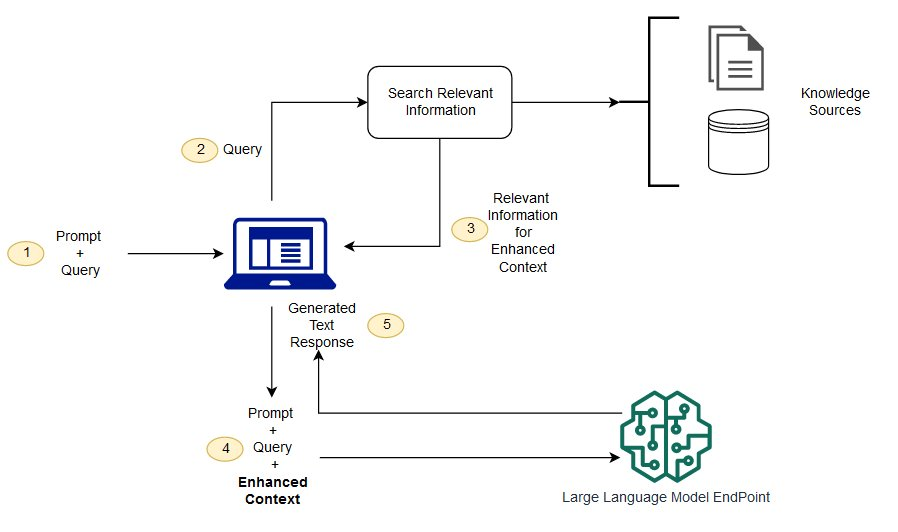
\includegraphics[scale=0.618]{pix/rag/jumpstart-fm-rag.jpg}
%\caption{}
\label{fig:jumpstart-fm-rag}
\end{figure}

\subsection{What is the difference between Retrieval-Augmented Generation and semantic search?}

Semantic search enhances RAG results for organizations wanting to add vast external knowledge sources 
to their LLM applications. Modern enterprises store vast amounts of information like manuals, FAQs, 
research reports, customer service guides, and human resource document repositories across various 
systems. Context retrieval is challenging at scale and consequently lowers generative output quality.

Semantic search technologies can scan large databases of disparate information and retrieve data more 
accurately. For example, they can answer questions such as, "How much was spent on machinery repairs 
last year?” by mapping the question to the relevant documents and returning specific text instead of 
search results. Developers can then use that answer to provide more context to the LLM.

Conventional or keyword search solutions in RAG produce limited results for knowledge-intensive tasks. 
Developers must also deal with word embeddings, document chunking, and other complexities as they manually 
prepare their data. In contrast, semantic search technologies do all the work of knowledge base preparation 
so developers don't have to. They also generate semantically relevant passages and token words ordered 
by relevance to maximize the quality of the RAG payload.





%+++++++++++++++++++++++++++++++++++++++++++
\section{References}
%-------------------------------------------

Retrieval-Augmented Generation (RAG) is a framework that combines retrieval-based and generation-based approaches for natural language processing tasks. Here are some notable research papers on RAG and related topics:

\begin{itemize}
%\setlength{\itemsep}{0pt}
%\setlength{\parsep}{0pt}
\setlength{\parskip}{0pt}
\item[1.]
{\bf "Retrieval-Augmented Generation for Knowledge-Intensive NLP Tasks"}

   Authors: Patrick Lewis, Ethan Perez, Aleksandra Piktus, Fabio Petroni, Vladimir Karpukhin, Naman Goyal, Heinrich Küttler, Mike Lewis, Wen-tau Yih, Tim Rocktäschel, Sebastian Riedel, Douwe Kiela  
   
   Year: 2020  
   
   Summary: This paper presents the RAG model, which integrates a retriever (a dense passage retriever) with a generator (a pre-trained sequence-to-sequence model like BART or T5) to answer knowledge-intensive questions. By incorporating external knowledge retrieval into the generation process, RAG can produce more accurate and informative responses.

\item[2.]

{\bf "Dense Passage Retrieval for Open-Domain Question Answering"}

   Authors: Vladimir Karpukhin, Barlas Oguz, Sewon Min, Patrick Lewis, Ledell Wu, Sergey Edunov, Danqi Chen, Wen-tau Yih  
   
   Year: 2020  
   
   Summary: Although not solely about RAG, this paper introduces Dense Passage Retrieval (DPR), an essential component used in RAG models for retrieving relevant documents. DPR is based on dense embeddings learned through a dual-encoder framework optimized for open-domain question answering tasks.

\item[3.]

{\bf "Improving Open Domain Dialogue Systems via Knowledge Graph Based Synthetic Corpus Generation"}

   Authors: Harsh Jhamtani, Peter J. Liu, Luke Zettlemoyer  
   
   Year: 2021  
   
   Summary: This paper discusses enhancing dialogue systems using external knowledge sources. While not exclusively about RAG, it highlights the importance of retrieval in dialogue systems and discusses approaches to integrate retrieval with generation.
\end{itemize}

These papers provide a foundational understanding of RAG and its components, as well as related advancements in retrieval-based NLP techniques. For the most up-to-date research, you may also want to search for recent publications in venues like ACL, EMNLP, or NeurIPS, where developments on retrieval-augmented models are frequently presented.

